\documentclass[../main.tex]{subfiles}

\begin{document}


\chapter{Fourier Analysis}
\textbf{CHAPTER OBJECTIVES}

\noindent The primary objective of this chapter is to introduce you to Fourier analysis. The
subject, which is named after Joseph Fourier, involves identifying cycles or patterns
within a time series of data. Specific objectives and topics covered in this chapter are

\begin{itemize}
	\item Understanding sinusoids and how they can be used for curve fitting.
	\item Knowing how to use least-squares regression to fit a sinusoid to data.
	\item Knowing how to fit a Fourier series to a periodic function.
	\item Understanding the relationship between sinusoids and complex exponentials
	based on Euler's formula.
	\item Recognizing the benefits of analyzing mathematical function or signals in the frequency domain (i.e., as a function of frequency).
	\item Understanding how the Fourier integral and transform extend Fourier analysis to aperiodic functions.
	\item Understanding how the discrete Fourier transform (DFT) extends Fourier analysis
	to discrete signals.
	\item Recognizing how discrete sampling affects the ability of the DFT to distinguish
	frequencies. In particular, know how to compute and interpret the Nyquist
	frequency.
	\item Recognizing how the fast Fourier transform (FFT) provides a highly efficient
	means to compute the DFT for cases where the data record length is a power of 2.
	\item Knowing how to use the MATLAB function \texttt{fft} to compute a DFT and
	understand how to interpret the results.
	\item Knowing how to compute and interpret a power spectrum.
\end{itemize}

\noindent\textbf{YOU'VE GOT A PROBLEM}\\

\noindent At the begginning of Chap. 8, we used Newton's second law and force balances to predict the equilibrium positions of three bungee jumpers connected by cords. Then, in Chap. 13, we determined the same systems's eigenvalues and eigenvectors in order to identify its resonant frequences and principal modes of vibration.
Although this analysis certainly provided useful results, it required detailed system information including
knowledge of the underlying model and parameters (i.e., the jumpers' masses and the
cords' spring constants).

So suppose that you have measurements of the jumpers' positions or velocities at discrete, equally spaced times (recall Fig. 13.1). Such information is referred to as a \textit{time series}. However, suppose further that you do not know the underlying model or the parameters needed to compute the eigenvalues. For such cases, is there any way to use the time
series to learn something fundamental about the system's dynamics?

In this chapter, we describe such an approach, \textit{Fourier analysis}, which provides a way to accomplish this objective. The approach is based on the premise that more complicated functions (e.g., a time series) can be represented by the sum of simpler trigonometric functions. As a prelude to outlining how this is done, it is useful to explore how data can be fit
with sinusoidal functions.

\label{cha:cha_P_16_1}
\section{CURVE FITTING WITH SINUSOIDAL FUNCTIONS}

\noindent A periodic function $f(t)$ is one for which

\begin{equation}
	\tag{16.1}
	f(t) = f(t + T)
\end{equation}

\noindent where T is a constant called the \textit{period} that is the smallest value of time for which Eq. (16.1) holds. Common examples include both artificial and natural signals (Fig. 16.1a).

\begin{figure}[H]
	\centering
	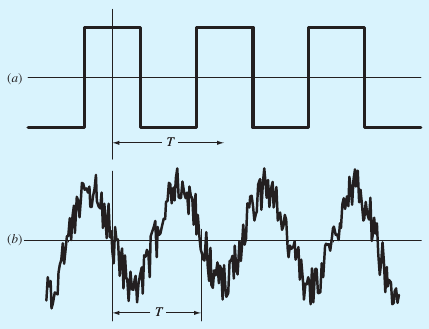
\includegraphics[width=1\linewidth]{fig_16_1}
	\caption{\textsf{Aside from trigonometric functions such as sines and cosines, periodic functions include
	idealized waveforms like the square wave depicted in (a). Beyond such artificial forms, periodic
	signals in nature can be contaminated by noise like the air temperatures shown in (b).}}
	\label{fig:fig_16_1}
\end{figure}

\begin{figure}[H]
	\centering
	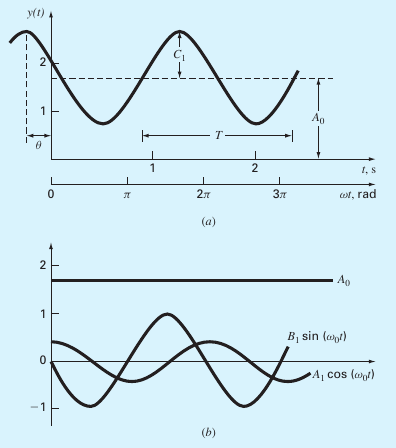
\includegraphics[width=1\linewidth]{fig_16_2}
	\caption{\textsf{(a) A plot of the sinusoidal function $y(t) = A_0 + C_1 \cos(\omega_0 t + \theta)$. For this case, $A_0 = 1.7$, $C_1 = 1$, $\omega_0 = 2 \pi / T = 2 \pi / (1.5 s)$, and $\theta = \pi / 3$ radians $= 1.0472$ ($= 0.25 s$). Other	parameters used to describe the curve are the frequency $f = \omega_0 /(2\pi)$, which or this case is 1 cycle $/ (1.5 s) = 0.6667$ Hz and the period $T = 1.5 s$. (b) An alternative expression of the same curve is $y(t) = A_0 + A_1 \cos(\omega_0 t) + B_1 \sin(\omega_0 t)$. The three components of this function are depicted in (b), where $A_1 = 0.5$ and $B_1 = -0.866$. The summation of the three curves in (b) yields the single curve in (a).}}
	\label{fig:fig_16_2}
\end{figure}

The most fundamental are sinusoidal functions. In this discussion, we will use the term \textit{sinusoid} to represent any waveform that can be described as a sine or cosine. There is no clear-cut convention for choosing either function, and in any case, the results will be identical because the two functions are simply offset in time by $\pi/2$ radians. For this chapter, we will use the cosine, which can be expressed generally as

\begin{equation}
	\tag{16.2}
	f(t) = A_0 + C_1 \cos (\omega_0 t + \theta)
\end{equation}

\noindent Inspection of Eq. (16.2) indicates that four parameters serve to uniquely characterize the
sinusoid (Fig. 16.2a):

\begin{itemize}
	\item The \textit{mean value} $A_0$ sets the average height above the abscissa.
	\item The \textit{amplitude} $C_1$ specifies the height of the oscillation.
	\item The \textit{angular frequency} $\omega_0$ characterizes how often the cycles occur.
	\item The \textit{phase angle} (or \textit{phase shift}) $\theta$ parameterizes the extent to which the sinusoid is shifted horizontally.
\end{itemize}

\begin{figure}[H]
	\centering
	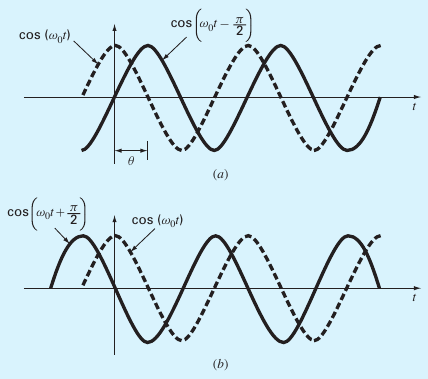
\includegraphics[width=1\linewidth]{fig_16_3}
	\caption{\textsf{Graphical depictions of (a) a lagging phase angle and (b) a leading phase angle. Note that the lagging curve in (a) can be alternatively described as $\cos(\omega_0 t + 3 \pi /2)$. In other words, if a curve lags by an angle of $\alpha$, it can also be represented as leading by $2\pi - \alpha$.}}
	\label{fig:fig_16_3}
\end{figure}

Note that the \textit{angular frequency} (in radians/time) is related to the \textit{ordinary frequency} $f$ (in cycles/time) by 

\begin{equation}
	\tag{16.3}
	\omega_0 = 2 \pi f
\end{equation}

\noindent and the ordinary frequency in turn is related to the period $T$ by

\begin{equation}
	\tag{16.4}
	f = \frac{1}{T}
\end{equation}

In addition, the \textit{phase angle} represents the distance in radians from $t = 0$ to the point at which the cosine function begins a new cycle. As depicted in Fig. 16.3a, a negative value is referred to as a \textit{lagging phase angle} because the curve $\cos(\omega_0 t - \theta)$ begins a new cycle $\theta$ radians after $\cos(\omega_0 t)$. Thus, $\cos(\omega_0 t - \theta)$ is said to lag $\cos(\omega_0 t)$. Conversely, as in Fig. 16.3b, a positive value is referred to as a \textit{leading phase angle}.

Although Eq. (16.2) is an adequate mathematical characterization of a sinusoid, it is awkward to work with from the standpoint of curve fitting because the phase shift is included in the argument of the cosine function. This deficiency can be overcome by invoking the trigonometric identity:

\begin{equation}
	\tag{16.5}
	C_1 \cos(\omega_0 t + \theta) = C_1 [\cos(\omega_0 t + \theta) \cos(\theta) - \sin(\omega_0 t + \theta) \sin(\theta)]
\end{equation}

\noindent Substituting Eq. (16.5) into Eq. (16.2) and collecting terms gives (Fig. 16.2b)

\begin{equation}
	\tag{16.6}
	f(t) = A_0 + A_1 \cos(\omega_0 t) + B_1 \sin(\omega_0 t)
\end{equation}

\noindent where

\begin{equation}
	\tag{16.7}
	A_1 = C_1 \cos(\theta) \quad \quad B_1 = - C_1 \sin(\theta)
\end{equation}

\noindent Dividing the two parts of Eq. (16.7) gives

\begin{equation}
	\tag{16.8}
	\theta = \arctan (- \frac{B_1}{A_1})
\end{equation}

\noindent where, if $A_1 < 0$, add $\pi$ to $\theta$. Squaring and summing Eq. (16.7) leads to

\begin{equation}
	\tag{16.9}
	C_1 = \sqrt{A^2_1 + B ^2_1}
\end{equation}

\noindent Thus, Eq. (16.6) represents an alternative formulation of Eq. (16.2) that still requires four parameters but that is cast in the format of a general linear model [recall Eq. (15.7)]. As we will
discuss in the next section, it can be simply applied as the basis for a least-squares fit.

Before proceeding to the next section, however, we should stress that we could have
employed a sine rather than a cosine as our fundamental model of Eq. (16.2). For example,

\begin{equation}
	\notag
	f(t) = A_0 + C_1 \sin(\omega_0 t + \delta)
\end{equation}

\noindent could have been used. Simple relationships can be applied to convert between the two forms:

\begin{equation}
	\notag
	\sin(\omega_0 t + \delta) = \cos(\omega_0 t + \delta - \frac{\pi}{2})
\end{equation}

\noindent and

\begin{equation}
	\tag{16.10}
	\sin(\omega_0 t + \delta) = \sin(\omega_0 t + \delta + \frac{\pi}{2})
\end{equation}

\noindent In other words, $\theta = \delta - \pi/2$. The only important consideration is that one or the other format
should be used consistently. Thus, we will use the cosine version throughout our discussion.

\label{cha:cha_P_16_1_1}
\subsection{Least-Squares Fit of a Sinusoid}

\noindent Equation (16.6) can be thought of as a linear least-squares model:

\begin{equation}
	\tag{16.11}
	y = A_0 + A_1 \cos(\omega_0 t) + B_1 \sin(\omega_0 t) + e
\end{equation}

\noindent which is just another example of the general model [recall Eq. (15.7)]

\begin{equation}
	\notag
	y = a_0 z_0 + a_1 z_1 + a_2 z_2 + \cdots + a_m z_m + e
\end{equation}

\noindent where $z_0 = 1$, $z_1 = \cos(\omega_0 t)$, $z_2 = sin(\omega_0 t)$, and all other $z$'s = 0. Thus, our goal is to determine coefficient values that minimize

\begin{equation}
	\notag
	S_r = \sum ^ N _ {i=1} \{ y_i - [A_0 + A_1 \cos(\omega_0 t) + B_1 \sin(\omega_0 t)]\}^2
\end{equation}

\noindent The normal equations to accomplish this minimization can be expressed in matrix form as [recall Eq. (15.10)]

\begin{equation}
	\tag{16.12}
	\begin{bmatrix}
		N & \sum \ cos(\omega_0 t) & \sum \sin(\omega_0 t) \\
		\sum \cos(\omega_0 t) & \sum \cos^2 (\omega_0 t) & \sum \cos (\omega_0 t) \sin (\omega_0 t) \\
		\sum \sin(\omega_0 t) & \sum \cos (\omega_0 t) \sin (\omega_0 t) & \sin^2 (\omega_0 t)
	\end{bmatrix}
	\begin{Bmatrix}
		A_0 \\ B_1 \\ B_1
	\end{Bmatrix}
	=
	\begin{Bmatrix}
		\sum y \\ \sum y \cos(\omega_0 t) \\ \sum y \sin(\omega_0 t)
	\end{Bmatrix}
\end{equation}
% 385

These equations can be employed to solve for the unknown coefficients. However,
rather than do this, we can examine the special case where there are N observations equispaced at intervals of $\Delta t$ and with a total record length of $T = (N - 1)\Delta t$. For this situa-
tion, the following average values can be determined (see Prob. 16.3):

\begin{equation}
	\tag{16.13}
	\begin{matrix}
		\frac{\sum \sin (\omega_0 t)}{N} = 0 & \frac{\sum \cos (\omega_0 t)}{N} = 0 \\
		\frac{\sum \sin ^2 (\omega_0 t)}{N} = \frac{1}{2} & \frac{\sum \cos ^2 (\omega_0 t)}{N} = \frac{1}{2} \\
		\frac{\sum \cos (\omega_0 t) \sin(\omega_0 t)}{N} = 0
	\end{matrix}
\end{equation}

\noindent Thus, for equispaced points the normal equations become

\begin{equation}
	\notag
	\begin{bmatrix}
		N & 0 & 0 \\
		0 & N/2 & 0 \\
		0 & 0 & N/2
	\end{bmatrix}
	\begin{Bmatrix}
		A_0 \\ B_1 \\ B_2
	\end{Bmatrix}
	=
	\begin{bmatrix}
		\sum y \\
		\sum y \cos(\omega_0 t) \\
		\sum y \sin(\omega_0 t)
	\end{bmatrix}
\end{equation}

\noindent The inverse of a diagonal matrix is merely another diagonal matrix whose elements are the
reciprocals of the original. Thus, the coefficients can be determined as

\begin{equation}
	\notag
	\begin{Bmatrix}
		A_0 \\ B_1 \\ B_2
	\end{Bmatrix}
	=
	\begin{bmatrix}
		1/N & 0 & 0 \\
		0 & 2/N & 0 \\
		0 & 0 & 2/N
	\end{bmatrix}
	\begin{bmatrix}
		\sum y \\
		\sum y \cos(\omega_0 t) \\
		\sum y \sin(\omega_0 t)
	\end{bmatrix}
\end{equation}

\noindent or

\begin{equation}
	\tag{16.14}
	A_0 = \frac{\sum y}{N}
\end{equation}

\begin{equation}
	\tag{16.15}
	A_1 =\frac{2}{N} \sum y \cos(\omega_0 t)
\end{equation}

\begin{equation}
	\tag{16.16}
	B_1 = \frac{2}{N} \sum y \sin(\omega_0 t)
\end{equation}

\noindent Notice that the first coefficient represents the function's average value.

\begin{example} Least-Squares Fit of a Sinusoid

    \noindent\textbf{Problem Statement.}\quad The curve in Fig. 16.2a is described by $y = 1.7 + \cos(4.189t + 1.0472)$. Generate 10 discrete values for this curve at intervals of $\Delta t = 0.15$ for the range
	t = 0 to 1.35. Use this information to evaluate the coefficients of Eq. (16.11) by a least squares fit.

    \noindent\textbf{Solution.}\quad  The data required to evaluate the coefficients with $\omega = 4.189$ are

	\noindent
	\begin{tabular}{c c c c}
		\textbf{t} & \textbf{y} & \textbf{$y \cos(\omega_0 t)$} & \textbf{$y \sin(\omega_0 t)$} \\
		\hline
		0 & 2.200 & 2.200 & 0.000 \\
		0.15 & 1.595 & 1.291 & 0.938 \\
		0.30 & 1.031 & 0.319 & 0.980 \\
		0.45 & 0.722 & -0.223 & 0.687 \\
		0.60 & 0.786 & -0.636 & 0.462 \\
		0.75 & 1.200 & -1.200 & 0.000 \\
		0.90 & 1.805 & -1.460 & -1.061 \\
		1.05 & 2.369 & -0.732 & -2.253 \\
		1.20 & 2.678 & 0.829 & -2.547 \\
		1.35 & 2.614 & 2.114 & -1.536 \\
		\hline
		$\sum$ = & 17.000 & 2.502 & -4.330
	\end{tabular}

	\noindent These results can be used to determine [Eqs. (16.14) through (16.16)]

	$$
		A_0 = \frac{17.000}{10} = 1.7	\quad A_1 = \frac{2}{10} 2.502 = 0.500 \quad B_1 = \frac{2}{10} (-4.330) = -0.866
	$$

	\noindent Thus, the least-squares fit is

	$$
		y = 1.7 + 0.500 \cos(\omega_0 t) - 0.866 \sin(\omega_0 t)
	$$

	\noindent The model can also be expressed in the format of Eq. (16.2) by calculating [Eq. (16.8)]

	$$
		\theta = \arctan (\frac{-0.866}{0.500}) = 1.0472
	$$

	\noindent and [Eq. (16.9)]

	$$
		C_1 = \sqrt{0.5^2 + (-0.866)^2} = 1.00
	$$

	\noindent to give 

	$$
		y = 1.7 + \cos(\omega_0 t + 1.0472)
	$$

	\noindent or alternatively, as a sine by using [Eq. (16.10)]

	$$
		y = 1.7 + \sin (\omega_0 t + 2.618)
	$$
\end{example}

The foregoing analysis can be extended to the general model
\begin{equation}
	\notag
	f(t) = A_0 + A_1 \cos(\omega_0 t) + B_1 \sin(\omega_0 t) + A_2 \cos(2 \omega_0 t) + B_2 \sin(2 \omega_0 t) + \cdots + A_m \cos(m \omega_0 t) + B_m \sin(m \omega_0 t)
\end{equation}

\noindent where, for equally spaced data, the coefficients can be evaluated by

\begin{equation}
	\notag
	A_0 = \frac{\sum y}{N}
\end{equation}

\begin{equation}
	\notag
	\left.
		\begin{array}{ll}
			A_j = \frac{2}{N} \sum y \cos(j \omega_0) t \\
			B_j = \frac{2}{N} \sum y \sin(j \omega_0 t)
		\end{array}
	\right \} j = 1,2, \dotsb , m
\end{equation}

%387
Although these relationships can be used to fit data in the regression sense (i.e.,$N  > 2 m + 1$), an alternative application is to employ them for interpolation or collocation - that
is, to use them for the case where the number of unknowns $2m + 1$ is equal to the number
of data points $N$. This is the approach used in the continuous Fourier series, as described
next.

\label{cha:cha_P_16_2}
\section{CONTINUOUS FOURIER SERIES}

In the course of studying heat-flow problems, Fourier showed that an arbitrary periodic
function can be represented by an infinite series of sinusoids of harmonically related
frequencies. For a function with period $T$, a continuous Fourier series can be written

\begin{equation}
	\notag
	f(t) a_0 + a_1 \cos(\omega_0 t) + b_1 \sin(\omega_0 t) +  a_2 \cos(2 \omega_0 t) + b_2 \sin(2 \omega_0 t) + \cdots
\end{equation}

\noindent or more concisely,

\begin{equation}
	\tag{16.17}
	f(t) = a_0 + \sum ^ \infty _ {k=1} [a_k \cos(k \omega_0 t) + b_k \sin(k \omega_0 t)]
\end{equation}

\noindent where the angular frequency of the first mode $(\omega_0 = 2 \pi /T)$ is called the fundamental
frequency and its constant multiples $2 \omega_0, 3 \omega_0$, etc., are called harmonics. Thus, Eq. (16.17)
expresses $f(t)$ as a linear combination of the basis functions: $1, cos( \omega_0 t), sin(\omega_0 t), cos(2 \omega_0 t),
sin(2 \omega_0 t), \dots$

The coefficients of Eq. (16.17) can be computed via

\begin{equation}
	\tag{16.18}
	a_k = \frac{2}{T} \int ^ T _ 0 f(t) \cos (k \omega_0 t) dt
\end{equation}

\noindent and

\begin{equation}
	\tag{16.19}
	b_k = \frac{2}{T} \int ^ T _ 0 f(t) \sin (k \omega_0 t) dt
\end{equation}

\noindent for $k = 1, 2, \dots$ and

\begin{equation}
	\tag{16.20}
	a_0 = \frac{1}{T} \int ^ T _ 0 f(t)dt
\end{equation}

\begin{example} Continuous Fourier Series Approximation

    \noindent\textbf{Problem Statement.}\quad Use the continuous Fourier series to approximate the square or rectangular wave function (Fig. 16.1a) with a height of 2 and a period $T = 2\pi /\omega_0$:

	$$
		f(t) = \left\{ \begin{matrix}
			-1 & -T/2 < t < -T/4 \\
			1 & -T/4 < t < T/4 \\
			-1 & T/4 < t < T/2
		\end{matrix}  \right.
	$$

    \noindent\textbf{Solution.}\quad  Because the average height of the wave is zero, a value of $a_0 = 0$ can be
	obtained directly. The remaining coefficients can be evaluated as [Eq. (16.18)]

	$$
		a_k = \frac{2}{T} \int_{-T/s} ^{T/2} f(t) \cos (k \omega_0 t) dt = \frac{2}{T} [- \int ^ {-T/4} _ {-T/2} \cos(k \omega_0 t) dt + \int ^ {T/4} _ {-T/4} \cos (k \omega_0 t) dt - \int _ {T/4} ^ {T/2} \cos(k \omega_0 t) dt]
	$$

	\noindent The integrals can be evaluated to give

	$$
		a_k = \left\{ \begin{matrix}
			4 / (k \pi) & \text{for } k = 1,5,9, \dots \\
			-4 / (k \pi) & \text{for } k = 3,7,11, \dots \\
			0 & \text{for } k = \text{even integers} \dots \\
		\end{matrix} \right.
	$$

	\begin{figure}[H] 
		\centering
		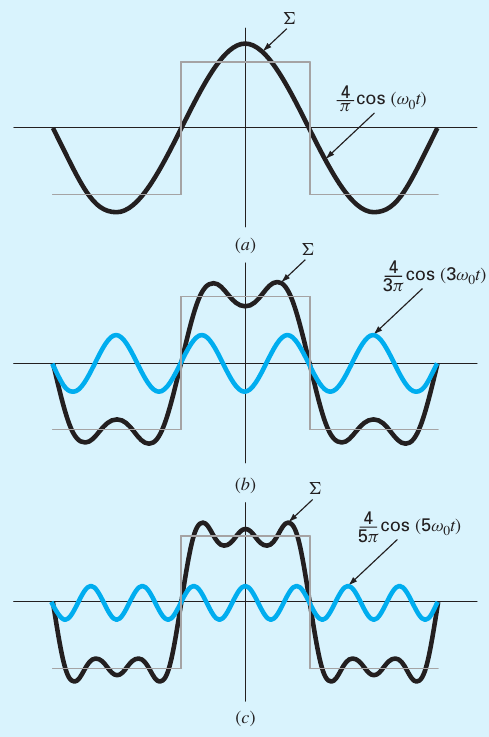
\includegraphics[width=1\linewidth]{fig_16_4}
		\caption{\textsf{The Fourier series approximation of a square wave. The series of plots shows the summation up
		to and including the (a) first, (b) second, and (c) third terms. The individual terms that were
		added or subtracted at each stage are also shown.}}
		\label{fig:fig_16_4}
	\end{figure}

	\noindent Similarly, it can be determined that all the $b$'s = 0. Therefore, the Fourier series approximation is

	$$
		f(t) = \frac{4}{\pi} \cos(\omega_0 t) - \frac{4}{3 \pi} \cos(3 \omega_0 t) + \frac{4}{5 \pi} \cos(5 \omega_0 t) - \frac{4}{7 \pi} \cos (7 \omega_0 t) + \dots
	$$

	\noindent The results up to the first three terms are shown in Fig. 16.4.
\end{example}


Before proceeding, the Fourier series can also be expressed in a more compact form
using complex notation. This is based on \textit{Euler's formula} (Fig. 16.5):

\begin{equation}
	\tag{16.21}
	e^{\pm ix} = \cos x \pm  i \sin x
\end{equation}

\noindent where $i = \sqrt{-1}$, and $x$ is in radians. Equation (16.21) can be used to express the Fourier
series concisely as (Chapra and Canale, 2010)

\begin{equation}
	\tag{16.22}
	f(t) = \sum _ {k=-\infty} ^ {\infty} \tilde{c}_k e^{i k \omega_0 t} 
\end{equation}

\noindent where the coefficients are

\begin{equation}
	\tag{16.23}
	\tilde{c}_k = \frac{1}{T} \int ^ {T/2} _ {-T/2} f(t) e ^ {-ik \omega_0 t} dt
\end{equation}

Note that the tildes ~ are included to stress that the coefficients are complex numbers.
Because it is more concise, we will primarily use the complex form in the rest of the
chapter. Just remember, that it is identical to the sinusoidal representation.

\begin{figure}[H] % FIXME too huge
	\centering
	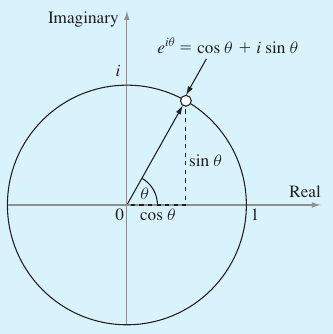
\includegraphics[width=1\linewidth]{fig_16_5}
	\caption{\textsf{Graphical depiction of Euler's formula. The rotating vector is called a phasor.}}
	\label{fig:fig_16_5}
\end{figure}

\label{cha:cha_P_16_3} %390
\section{FREQUENCY AND TIME DOMAINS}

\noindent To this point, our discussion of Fourier analysis has been limited to the \textit{time domain}. We
have done this because most of us are fairly comfortable conceptualizing a function's
behavior in this dimension. Although it is not as familiar, the \textit{frequency domain} provides an
alternative perspective for characterizing the behavior of oscillating functions.

Just as amplitude can be plotted versus time, it can also be plotted versus frequency.
Both types of expression are depicted in Fig. 16.6a, where we have drawn a threedimensional graph of a sinusoidal function:

\begin{equation}
	\notag
	f(t) = C_1 \cos(t + \frac{\pi}{2})
\end{equation} 

\begin{figure}[H] 
	\centering
	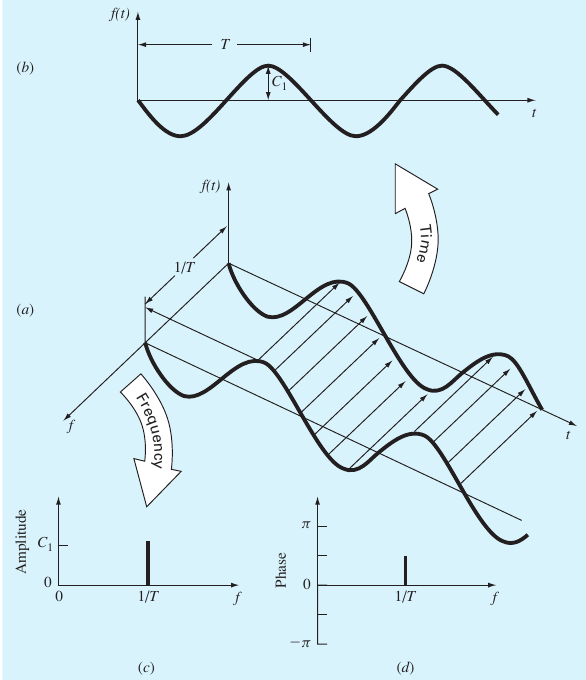
\includegraphics[width=1\linewidth]{fig_16_6}
	\caption{\textsf{(a) A depiction of how a sinusoid can be portrayed in the time and the frequency domains. The
	time projection is reproduced in (b), whereas the amplitude-frequency projection is reproduced in
	(c). The phase-frequency projection is shown in (d).}}
	\label{fig:fig_16_6}
\end{figure}

\noindent In this plot, the magnitude or amplitude of the curve $f(t)$ is the dependent variable, and time $t$
and frequency $f = \omega_0 / 2 \pi$ are the independent variables. Thus, the amplitude and the time
axes form a \textit{time plane}, and the amplitude and the frequency axes form a \textit{frequency plane}.
The sinusoid can, therefore, be conceived of as existing a distance $1/T$ out along the frequency axis and running parallel to the time axes. Consequently, when we speak about the
behavior of the sinusoid in the time domain, we mean the projection of the curve onto the
time plane (Fig. 16.6b). Similarly, the behavior in the frequency domain is merely its projection onto the frequency plane.

As in Fig. 16.6c, this projection is a measure of the sinusoid's maximum positive
amplitude $C_1$. The full peak-to-peak swing is unnecessary because of the symmetry.
Together with the location $1/T$ along the frequency axis, Fig. 16.6c now defines the
amplitude and frequency of the sinusoid. This is enough information to reproduce the
shape and size of the curve in the time domain. However, one more parameter - namely,
the phase angle - is required to position the curve relative to $t = 0$. Consequently, a
phase diagram, as shown in Fig. 16.6d, must also be included. The phase angle is determined as the distance (in radians) from zero to the point at which the positive peak
occurs. If the peak occurs after zero, it is said to be delayed (recall our discussion of lags
and leads in Sec. 16.1), and by convention, the phase angle is given a negative sign.
Conversely, a peak before zero is said to be advanced and the phase angle is positive.
Thus, for Fig. 16.6, the peak leads zero and the phase angle is plotted as $+\pi / 2$. Figure 16.7 depicts some other possibilities.

We can now see that Fig. 16.6c and $d$ provide an alternative way to present or summarize the pertinent features of the sinusoid in Fig. 16.6a. They are referred to as \textit{line spectra}.
Admittedly, for a single sinusoid they are not very interesting. However, when applied to a
more complicated situation-say, a Fourier series-their true power and value is revealed.
For example, Fig. 16.8 shows the amplitude and phase line spectra for the square-wave
function from Example 16.2.

Such spectra provide information that would not be apparent from the time domain.
This can be seen by contrasting Fig. 16.4 and Fig. 16.8. Figure 16.4 presents two alternative time domain perspectives. The first, the original square wave, tells us nothing
about the sinusoids that comprise it. The alternative is to display these sinusoids-that
is, $(4 / \pi) \cos(\omega_0 t), -(4/3 \pi) \cos(3 \omega_0 t), (4/5 \pi) \cos(5 \omega_0t ),$ etc. This alternative does
not provide an adequate visualization of the structure of these harmonics. In contrast,
Fig. 16.8a and b provide a graphic display of this structure. As such, the line spectra
represent ``fingerprints'' that can help us to characterize and understand a complicated
waveform. They are particularly valuable for nonidealized cases where they sometimes
allow us to discern structure in otherwise obscure signals. In the next section, we will
describe the Fourier transform that will allow us to extend such analyses to nonperiodic
waveforms.

\label{cha:cha_P_16_4} %391
\section{FOURIER INTEGRAL AND TRANSFORM}

\noindent Although the Fourier series is a useful tool for investigating periodic functions, there are
many waveforms that do not repeat themselves regularly. For example, a lightning bolt
occurs only once (or at least it will be a long time until it occurs again), but it will cause interference with receivers operating on a broad range of frequencies - for example, TVs,
radios, and shortwave receivers. Such evidence suggests that a nonrecurring signal such as
that produced by lightning exhibits a continuous frequency spectrum. Because such phenomena are of great interest to engineers, an alternative to the Fourier series would be valuable for analyzing these aperiodic waveforms.

\begin{figure}[H] 
	\centering
	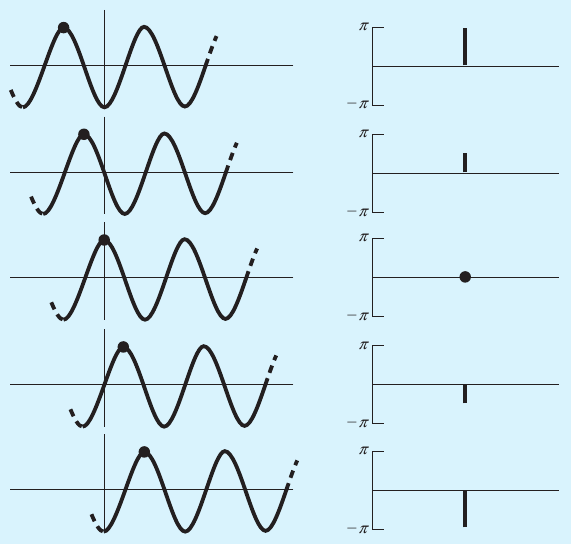
\includegraphics[width=1\linewidth]{fig_16_7}
	\caption{\textsf{Various phases of a sinusoid showing the associated phase line spectra.}}
	\label{fig:fig_16_7}
\end{figure}

The \textit{Fourier integral} is the primary tool available for this purpose. It can be derived
from the exponential form of the Fourier series [Eqs. (16.22) and (16.23)]. The transition
from a periodic to a nonperiodic function can be effected by allowing the period to approach infinity. In other words, as $T$ becomes infinite, the function never repeats itself and
thus becomes aperiodic. If this is allowed to occur, it can be demonstrated (e.g., Van
Valkenburg, 1974; Hayt and Kemmerly, 1986) that the Fourier series reduces to

\begin{equation}
	\tag{16.24}
	f(t) = \frac{1}{2 \pi} \int ^ \infty _ {-\infty} F(\omega) e ^ {i \omega t} d \omega
\end{equation}

\begin{figure}[H] 
	\centering
	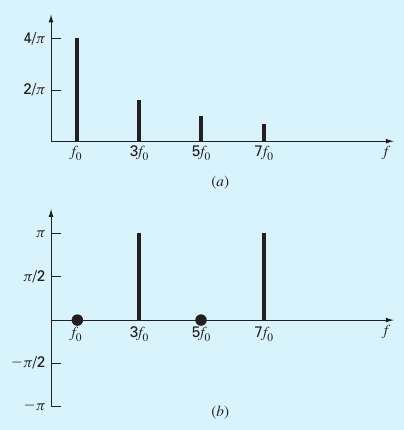
\includegraphics[width=1\linewidth]{fig_16_8}
	\caption{\textsf{(a) Amplitude and (b) phase line spectra for the square wave from Fig. 16.4.}}
	\label{fig:fig_16_8}
\end{figure}

\noindent and the coefficients become a continuous function of the frequency variable $\omega$, as in

\begin{equation}
	\tag{16.25}
	F(\omega) = \int ^ \infty _ {-\infty} f(t)e ^ {-i \omega t} dt
\end{equation}

The function $F(\omega)$, as defined by Eq. (16.25), is called the \textit{Fourier integral} of $f(t)$. In
addition, Eqs. (16.24) and (16.25) are collectively referred to as the \textit{Fourier transform}
pair. Thus, along with being called the Fourier integral, $F(\omega)$ is also called the \textit{Fourier
transform} of $f(t)$. In the same spirit, $f(t)$, as defined by Eq. (16.24), is referred to as the
\textit{inverse Fourier transform} of $F(\omega)$. Thus, the pair allows us to transform back and forth
between the time and the frequency domains for an aperiodic signal.

The distinction between the Fourier series and transform should now be quite clear.
The major difference is that each applies to a different class of functions-the series to periodic and the transform to nonperiodic waveforms. Beyond this major distinction, the two
approaches differ in how they move between the time and the frequency domains. The
Fourier series converts a continuous, periodic time-domain function to frequency-domain
magnitudes at discrete frequencies. In contrast, the Fourier transform converts a continuous time-domain function to a continuous frequency-domain function. Thus, the discrete
frequency spectrum generated by the Fourier series is analogous to a continuous frequency
spectrum generated by the Fourier transform.

Now that we have introduced a way to analyze an aperiodic signal, we will take the
final step in our development. In the next section, we will acknowledge the fact that a
signal is rarely characterized as a continuous function of the sort needed to implement
Eq. (16.25). Rather, the data are invariably in a discrete form. Thus, we will now show how
to compute a Fourier transform for such discrete measurements.

\label{cha:cha_P_16_5} %394
\section{DISCRETE FOURIER TRANSFORM (DFT)}

\noindent In engineering, functions are often represented by a finite set of discrete values. Additionally, data are often collected in or converted to such a discrete format. As depicted in
Fig. 16.9, an interval from 0 to $T$ can be divided into $n$ equispaced subintervals with widths
of $\Delta t = T /n$. The subscript $j$ is employed to designate the discrete times at which samples
are taken. Thus, $f_j$ designates a value of the continuous function $f(t)$ taken at $t_j$. Note that the
data points are specified at $j = 0, 1, 2, \dots , n - 1$. A value is not included at $j = n$. (See
Ramirez, 1985, for the rationale for excluding $f_n$.)

For the system in Fig. 16.9, a discrete Fourier transform can be written as
\begin{equation}
	\tag{16.26}
	F_k = \sum ^ {n-1} _ {j=0} f_j e ^ {-ik \omega_0 j} \quad \text{for } k=0 \text{ to } n - 1
\end{equation}

\noindent and the inverse Fourier transform as

\begin{equation}
	\tag{16.27}
	F_k = \frac{1}{n} \sum ^ {n-1} _ {k=0} F_k e ^ {ik \omega_0 j} \quad \text{for } j=0 \text{ to } n - 1
\end{equation}

\noindent where $\omega_0 = 2 \pi / n$.

\begin{figure}[H] 
	\centering
	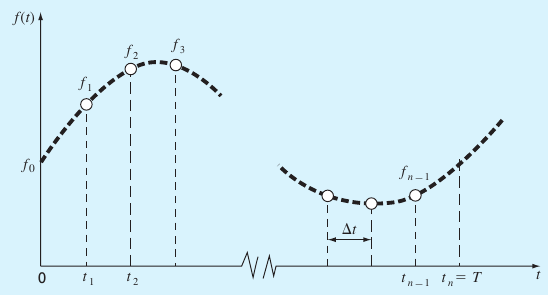
\includegraphics[width=1\linewidth]{fig_16_9}
	\caption{\textsf{The sampling points of the discrete Fourier series.}}
	\label{fig:fig_16_9}
\end{figure}

Equations (16.26) and (16.27) represent the discrete analogs of Eqs. (16.25) and
(16.24), respectively. As such, they can be employed to compute both a direct and an inverse Fourier transform for discrete data. Note that the factor $1/n$ in Eq. (16.27) is merely
a scale factor that can be included in either Eq. (16.26) or (16.27), but not both. For example, if it is shifted to Eq. (16.26), the first coefficient $F_0$ (which is the analog of the constant
$a_0$) is equal to the arithmetic mean of the samples.

Before proceeding, several other aspects of the DFT bear mentioning. The highest frequency that can be measured in a signal, called the \textit{Nyquist frequency}, is half the sampling
frequency. Periodic variations that occur more rapidly than the shortest sampled time interval cannot be detected. The lowest frequency you can detect is the inverse of the total
sample length.

As an example, suppose that you take 100 samples of data ($n = 100$ samples) at a
sample frequency of $f_s = 1000$ Hz (i.e., 1000 samples per second). This means that the
sample interval is

\begin{equation}
	\notag
	\Delta t = \frac{1}{f_s}=\frac{1}{1000 \text{ samples/s}} = 0.01 \text{ s/sample}
\end{equation}

\noindent The total sample length is 

\begin{equation}
	\notag
	t_n = \frac{n}{f_s} = \frac{100 \text{ samples}}{1000 \text{ samples/s}}=0.1 \text{ Hz}
\end{equation}

\noindent and the frequency increment is

\begin{equation}
	\notag
	\Delta f = \frac{f_s}{n} = \frac{1000 \text{ samples/s}}{100 \text{ samples}}=10 \text{ Hz}
\end{equation}

\noindent The Nyquist frequency is

\begin{equation}
	\notag
	f_{\text{max}} = 0.5 f_s = 0.5 (1000 \text{ Hz}) = 500 \text{ Hz}
\end{equation}

\noindent and the lowest detectable frequency is

\begin{equation}
	\notag
	f_{\text{min}} = \frac{1}{0.1 \text{s}} = 10 \text{ Hz}
\end{equation}

\noindent Thus, for this example, the DFT could detect signals with periods from $1/500 = 0.002 \text{s}$ up
to $1/10 = 0.1\text{s}$.

\label{cha:cha_P_16_5_1} % 395
\subsection{Fast Fourier Transform (FFT)}

\noindent Although an algorithm can be developed to compute the DFT based on Eq. (16.26), it is
computationally burdensome because $n^2$ operations are required. Consequently, for data
samples of even moderate size, the direct determination of the DFT can be extremely time
consuming.

\begin{figure}[H] 
	\centering
	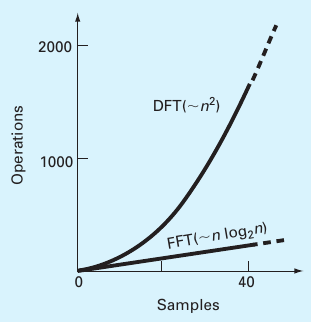
\includegraphics[width=1\linewidth]{fig_16_10}
	\caption{\textsf{Plot of number of operations vs. sample size for the standard DFT and the FFT.}}
	\label{fig:fig_16_10}
\end{figure}

The \textit{fast Fourier transform}, or \textit{FFT}, is an algorithm that has been developed to com-
pute the DFT in an extremely economical fashion. Its speed stems from the fact that it
utilizes the results of previous computations to reduce the number of operations. In particular, it exploits the periodicity and symmetry of trigonometric functions to compute
the transform with approximately $n \log_2n$ operations (Fig. 16.10). Thus, for $n = 50$ samples, the FFT is about 10 times faster than the standard DFT. For $n = 1000$, it is about
100 times faster.

The first FFT algorithm was developed by Gauss in the early nineteenth century
(Heideman et al., 1984). Other major contributions were made by Runge, Danielson,
Lanczos, and others in the early twentieth century. However, because discrete transforms
often took days to weeks to calculate by hand, they did not attract broad interest prior to the
development of the modern digital computer.

In 1965, J. W. Cooley and J. W. Tukey published a key paper in which they outlined an
algorithm for calculating the FFT. This scheme, which is similar to those of Gauss and
other earlier investigators, is called the Cooley-Tukey algorithm. Today, there are a host of
other approaches that are offshoots of this method. As described next, MATLAB offers a
function called \texttt{fft} that employs such efficient algorithms to compute the DFT.

\label{cha:cha_P_16_5_2} % 396
\subsection{MATLAB Function: \texttt{fft}}

\noindent MATLAB's \texttt{fft} function provides an efficient way to compute the DFT. A simple representation of its syntax is

\begin{lstlisting}[numbers=none]
	F = fft(f, n)
\end{lstlisting}

where \texttt{F =} a vector containing the DFT, and \texttt{f =} a vector containing the signal. The
parameter \texttt{n}, which is optional, indicates that the user wants to implement an $n$-point FFT.
If \texttt{f} has less than \texttt{n} points, it is padded with zeros and truncated if it has more.

Note that the elements in \texttt{F} are sequenced in what is called \textit{reverse-wrap-around
order}. The first half of the values are the positive frequencies (starting with the constant)
and the second half are the negative frequencies. Thus, if $n = 8$, the order is 0, 1, 2, 3, 4, -3, -2, -1. The following example illustrates the function's use to calculate the DFT of a
simple sinusoid.

\begin{example} Computing the DFT of a Simple Sinusoid with MATLAB

    \noindent\textbf{Problem Statement.}\quad Apply the MATLAB fft function to determine the discrete Fourier
	transform for a simple sinusoid:

	$$
		f(t) = 5 + \cos(2 \pi (12.5) t) + \sin(2 \pi (18.75) t)
	$$

	\noindent Generate 8 equispaced points with $\Delta t = 0.02 $s. Plot the result versus frequency.

    \noindent\textbf{Solution.}\quad  Before generating the DFT, we can compute a number of quantities. The sampling frequency is

	$$
		f_x = \frac{1}{\Delta t} = \frac{1}{0.02 s} = 50 \text{Hz}
	$$

	\noindent The total sample length is

	$$
		t_n = \frac{n}{f_s} = \frac{8 \text{samples}}{50 \text{samples/s}} = 0.16 s
	$$

	\noindent The Nyquist frequency is

	$$
		f_\text{max} 0.5 f_s = 0.5 (50Hz) = 25 \text{Hz}
	$$

	\noindent and the lowest detectable frequency is

	$$
		f_\text{min}	= \frac{1}{0.16 s} = 6.25 \text {Hz}
	$$

	\noindent Thus, the analysis can detect signals with periods from 1/25 = 0.04 s up to 1/6.25 = 0.16 s.
	So we should be able to detect both the 12.5 and 18.75 Hz signals.

	The following MATLAB statements can be used to generate and plot the sample
(Fig. 16.11a):

	\begin{lstlisting}[numbers=none]
		>> clc
		>> n=8; dt=0.02; fs=1/dt; T = 0.16;
		>> tspan=(0:n-1)/fs;
		>> y=5+cos(2*pi*12.5*tspan)+sin(2*pi*31.25*tspan);
		>> subplot(3,1,1);
		>> plot(tspan,y,'-ok','linewidth',2,'MarkerFaceColor','black');
		>> title('(a) f(t) versus time (s)');
	\end{lstlisting}

	\begin{figure}[H] 
		\centering
		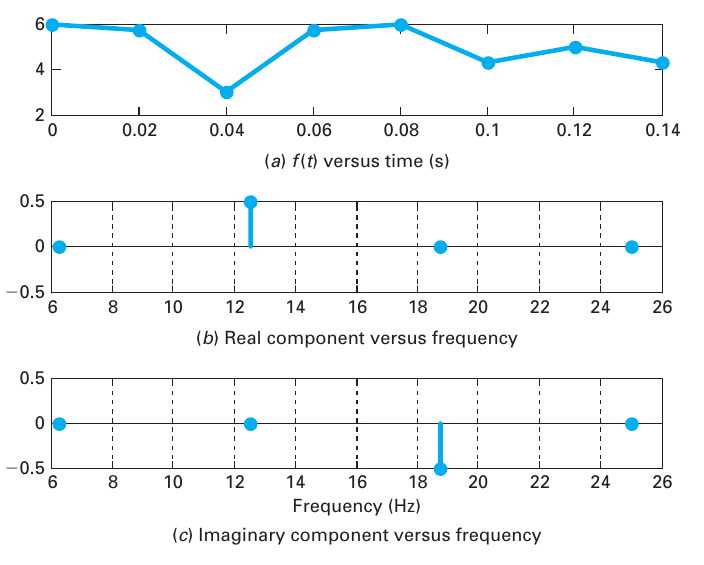
\includegraphics[width=1\linewidth]{fig_16_11}
		\caption{\textsf{Results of computing a DFT with MATLAB's \texttt{fft} function: (a) the sample; and plots of
		the (b) real and (c) imaginary parts of the DFT versus frequency.}}
		\label{fig:fig_16_11}
	\end{figure}

	\noindent As was mentioned at the beginning of Sec. 16.5, notice that tspan omits the last point.

	The \texttt{fft} function can be used to compute the DFT and display the results

	\begin{lstlisting}[numbers=none]
		>>Y=fft(y)/n;
		>>Y'
	\end{lstlisting}

	\noindent We have divided the transform by n in order that the first coefficient is equal to the arithmetic mean of the samples. When this code is executed, the results are displayed as

	\begin{lstlisting}[numbers=none]
		ans =
			5.0000
			0.0000 - 0.0000i
			0.5000
			-0.0000 + 0.5000i
			0
			-0.0000 - 0.5000i
			0.5000
			0.0000 + 0.0000i
	\end{lstlisting}

	\noindent Notice that the first coefficient corresponds to the signal's mean value. In addition, because of the \textit{reverse-wrap-around order}, the results can be interpreted as in the following
	table:

	\begin{tabular}{l l c c c c}
		\textbf{Index} & \textbf{k} & \textbf{Frequency} & \textbf{Period} & \textbf{Real} & \textbf{Imaginary} \\
		1 & 0 & constant & 5 & 0 \\
		2 & 1 & 6.25 & 0.16 & 0 & 0 \\
		3 & 2 & 12.5 & 0.08 & 0.5 & 0 \\
		4 & 3 & 18.75 & 0.053333 & 0 & 0.5 \\
		\textbf{5} & \textbf{4} & \textbf{25} & \textbf{0.04} & \textbf{0} & \textbf{0} \\
		6 & -3 & 31.25 & 0.032 & 0 & -0.5 \\
		7 & -2 & 37.5 & 0.026667 & 0.5 & 0 \\
		8 & -1 & 43.75 & 0.022857 & 0 & 0
	\end{tabular}

	\noindent Notice that the \texttt{fft} has detected the 12.5- and 18.75-Hz signals. In addition, we have highlighted the Nyquist frequency to indicate that the values below it in the table are redundant.
	That is, they are merely reflections of the results below the Nyquist frequency.

	If we remove the constant value, we can plot both the real and imaginary parts of the
DFT versus frequency

	\begin{lstlisting}[numbers=none]
		>> nyquist=fs/2;fmin=1/T;
		>> f = linspace(fmin,nyquist,n/2);
		>> Y(1)=[];YP=Y(1:n/2);
		>> subplot(3,1,2)
		>> stem(f,real(YP),'linewidth',2,'MarkerFaceColor','blue')
		>> grid;title('(b) Real component versus frequency')
		>> subplot(3,1,3)
		>> stem(f,imag(YP),'linewidth',2,'MarkerFaceColor','blue')
		>> grid;title('(b) Imaginary component versus frequency')
		>> xlabel('frequency (Hz)')
	\end{lstlisting}

	\noindent As expected (recall Fig. 16.7), a positive peak occurs for the cosine at 12.5 Hz
	(Fig. 16.11b), and a negative peak occurs for the sine at 18.75 Hz (Fig. 16.11c).
\end{example}

\label{cha:cha_P_16_6}
\section{THE POWER SPECTRUM}

\noindent Beyond amplitude and phase spectra, power spectra provide another useful way to discern
the underlying harmonics of seemingly random signals. As the name implies, it derives
from the analysis of the power output of electrical systems. In terms of the DFT, a \textit{power
spectrum} consists of a plot of the power associated with each frequency component versus
frequency. The power can be computed by summing the squares of the Fourier coefficients:

\begin{equation}
	\notag
	P_k = {|\tilde{c}_k|}^2
\end{equation}

\noindent where $P_k$ is the power associated with each frequency $k \omega_0$.

\begin{example}  Computing the Power Spectrum with MATLAB
	\noindent \textbf{Problem Statement. } \quad Compute the power spectrum for the simple sinusoid for which the
	DFT was computed in Example 16.3.

	\noindent \textbf{Solution. } \quad  The following script can be developed to compute the power spectrum:

	\begin{lstlisting}[numbers=none]
		% compute the DFT
		clc;clf
		n=8; dt=0.02;
		fs=1/dt;tspan=(0:n-1)/fs;
		y=5+cos(2*pi*12.5*tspan)+sin(2*pi*18.75*tspan);
		Y=fft(y)/n;
		f = (0:n-1)*fs/n;
		Y(1)=[];f(1)=[];
		% compute and display the power spectrum
		nyquist=fs/2;
		f = (1:n/2)/(n/2)*nyquist;
		Pyy = abs(Y(1:n/2)).^2;
		stem(f,Pyy,'linewidth',2,'MarkerFaceColor','blue')
		title('Power spectrum')
		xlabel('Frequency (Hz)');ylim([0 0.3])
	\end{lstlisting}

	\noindent As indicated, the first section merely computes the DFT with the pertinent statements from
	Example 16.3. The second section then computes and displays the power spectrum. As in
	Fig. 16.12, the resulting graph indicates that peaks occur at both 12.5 and 18.75 Hz as
	expected.

	\begin{figure}[H] 
		\centering
		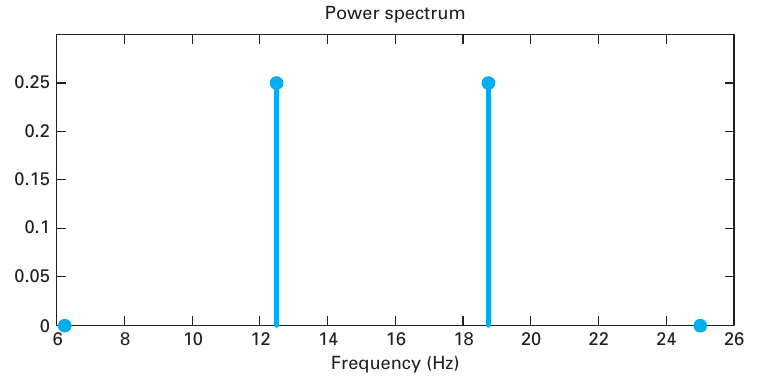
\includegraphics[width=1\linewidth]{fig_16_12}
		\caption{\textsf{Power spectrum for a simple sinusoidal function with frequencies of 12.5 and 18.75 Hz.}}
		\label{fig:fig_16_12}
	\end{figure}
\end{example}

\section[CASE STUDY: SUNSPOTS]{CASE STUDY: SUNSPOTS}
\noindent\textbf{Background.}\quad  In 1848, Johann Rudolph Wolf devised a method for quantifying solar
activity by counting the number of individual spots and groups of spots on the sun's surface. He computed a quantity, now called a \textit{Wolf sunspot number}, by adding 10 times the
number of groups plus the total count of individual spots. As in Fig. 16.13, the data set for
the sunspot number extends back to 1700. On the basis of the early historical records, Wolf
determined the cycle's length to be 11.1 years. Use a Fourier analysis to confirm this result
by applying an FFT to the data.

\noindent\textbf{Solution.}\quad  The data for year and sunspot number are contained in a MATLAB file,
\texttt{sunspot.dat}. The following statements load the file and assign the year and number information to vectors of the same name:

\begin{lstlisting}[numbers=none]
	>> load sunspot.dat
	>> year=sunspot(:,1);number=sunspot(:,2);
\end{lstlisting}

\noindent Before applying the Fourier analysis, it is noted that the data seem to exhibit an upward linear trend (Fig. 16.13). MATLAB can be used to remove this trend:

\begin{lstlisting}[numbers=none]
	>> n=length(number);
	>> a=polyfit(year,number,1);
	>> lineartrend=polyval(a,year);
	>> ft=number-lineartrend;
\end{lstlisting}

\noindent Next, the \texttt{fft} function is employed to generate the DFT

\begin{lstlisting}[numbers=none]
	F=fft(ft);
\end{lstlisting}

\noindent The power spectrum can then be computed and plotted

\begin{lstlisting}[numbers=none]
	fs=1;
	f=(0:n/2)*fs/n;
	pow=abs(F(1:n/2+1)).^2;
	plot(f,pow)
	xlabel('Frequency (cycles/year)'); ylabel('Power')
	title('Power versus frequency')
\end{lstlisting}

\begin{figure}[H] 
	\centering
	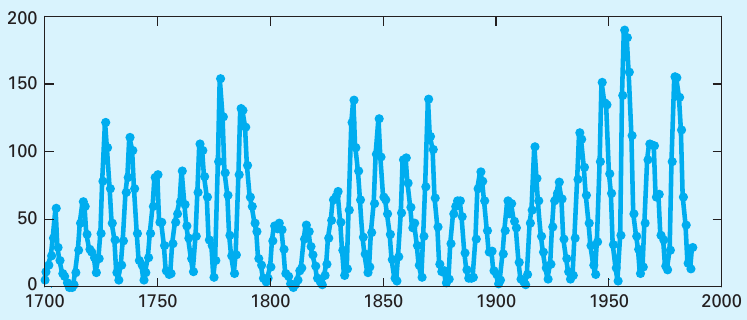
\includegraphics[width=1\linewidth]{fig_16_13}
	\caption{\textsf{Plot of Wolf sunspot number versus year. The dashed line indicates a mild, upward linear trend.}}
	\label{fig:fig_16_13}
\end{figure}

\begin{figure}[H] 
	\centering
	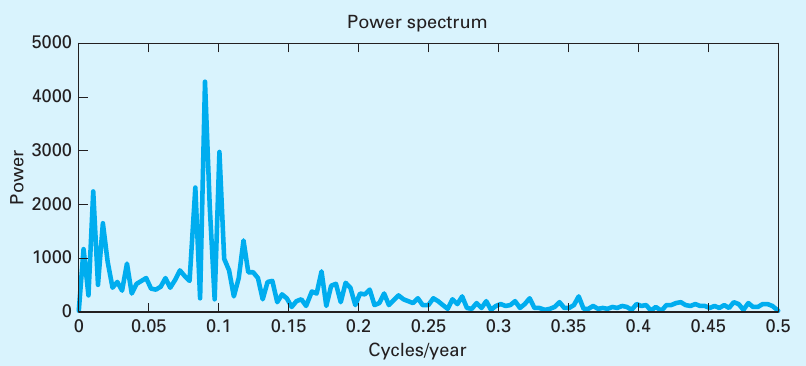
\includegraphics[width=1\linewidth]{fig_16_14}
	\caption{\textsf{Power spectrum for Wolf sunspot number versus year.}}
	\label{fig:fig_16_14}
\end{figure}

\noindent The result, as shown in Fig. 16.14, indicates a peak at a frequency of about 0.0915 Hz. This
corresponds to a period of 1/0.0915 = 10.93 years. Thus, the Fourier analysis is consistent
with Wolf's estimate of 11 years.

\noindent\textbf{PROBLEMS}
\begin{multicols}{2}
    \noindent\textbf{16.1} The pH in a reactor varies sinusoidally over the course
	of a day. Use least-squares regression to fit Eq. (16.11) to
	the following data. Use your fit to determine the mean,
	amplitude, and time of maximum pH. Note that the period
	is 24 hr

	\noindent
	\begin{tabular}{l c c c c c c}
		Time, hr & 0 & 2 & 4 & 5 & 7 & 9 \\
		pH & 7.6 & 7.2 & 7 & 6.5 & 7.5 & 7.2 \\
		Time, hr & 12 & 15 & 20 & 22 & 24 \\
		pH & 8.9 & 9.1 & 8.9 & 7.9 & 7
	\end{tabular}

	\noindent\textbf{16.2}  The solar radiation for Tucson, Arizona, has been tabulated as

	\noindent
	\begin{tabular}{l c c c c c c}
		Time, mo & J & F & M & A & M & J \\
		Radiation, W/m$^2$ & 144 & 188 & 245 & 311 & 351 & 359 \\
		Time, mo & J & A & S & O & N & D \\
		Radiation, W/m$^2$ & 308 & 287 & 260 & 211 & 159 & 131
	\end{tabular}

	\noindent Assuming each month is 30 days long, fit a sinusoid to these
	data. Use the resulting equation to predict the radiation in
	mid-August.

	\noindent\textbf{16.3} The average values of a function can be determined by

	$$
		\bar{f} = \frac{\int ^t _ 0 f(t) dt}{t}
	$$

	\noindent Use this relationship to verify the results of Eq. (16.13).

	\noindent\textbf{16.4} In electric circuits, it is common to see current
	behavior in the form of a square wave as shown in Fig. P16.4
	(notice that square wave differs from the one described in
	Example 16.2). Solving for the Fourier series from

	$$
		f(t) = \left\{ 
			\begin{matrix}
				A_0 & 0 \leq t \leq T/2 \\
				-A_0 & T/2 \leq t \leq T
			\end{matrix}
		\right.
	$$

	\noindent the Fourier series can be represented as

	$$
		f(t) = \sum ^ \infty _ {n=1} (\frac{4 A_0}{(2n -1) \pi}) \sin (\frac{2 \pi (2n -1) t}{T})
	$$

	\noindent Develop a MATLAB function to generate a plot of the first $n$
	terms of the Fourier series individually, as well as the sum of
	these six terms. Design your function so that it plots the
	curves from $t$ = 0 to $4T$. Use thin dotted red lines for the individual terms and a bold black solid line for the summation
	(i.e., 'k-','linewidth',2). The function's first line
	should be

	\noindent
	\begin{lstlisting}[numbers=none]
		function [t,f] = FourierSquare(A0,T,n)
	\end{lstlisting}

	\noindent Let $A_0 = 1$ and $T = 0.25$ s.

	\noindent\textbf{16.5} Use a continuous Fourier series to approximate the
	sawtooth wave in Fig. P16.5. Plot the first four terms along
	with the summation. In addition, construct amplitude and
	phase line spectra for the first four terms.

	\noindent\textbf{16.6}  Use a continuous Fourier series to approximate the tri-
	angular wave form in Fig. P16.6. Plot the first four terms
	along with the summation. In addition, construct amplitude
	and phase line spectra for the first four terms.

	\noindent
    \begin{minipage}{\linewidth}
        \centering
        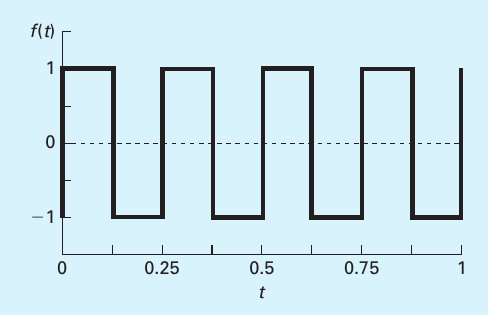
\includegraphics[width=0.8\linewidth]{./images/problem_16_4}
        \captionof*{figure}{Figure P16.4}
    \end{minipage}

	\noindent
    \begin{minipage}{\linewidth}
        \centering
        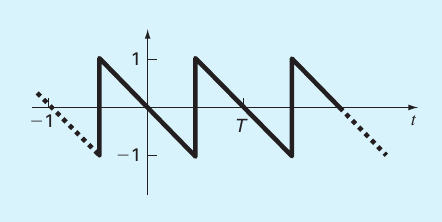
\includegraphics[width=0.8\linewidth]{./images/problem_16_5}
        \captionof*{figure}{Figure P16.5 \textsf{A sawtooth wave.}}
    \end{minipage}

	\noindent
    \begin{minipage}{\linewidth}
        \centering
        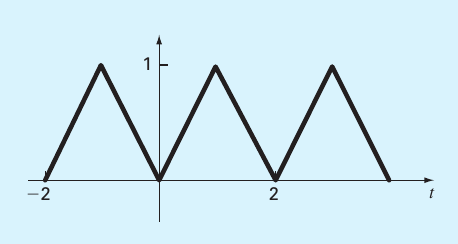
\includegraphics[width=0.8\linewidth]{./images/problem_16_6}
        \captionof*{figure}{Figure P16.6 \textsf{A triangular wave.}}
    \end{minipage}

	\noindent\textbf{16.7} Use the \textit{Maclaurin series expansions} for $e^x$, $\cos x$ and
	$\sin x$ to prove Euler's formula (Eq. 16.21).

	\noindent\textbf{16.8}A half-wave rectifier can be characterized by

	$$
		C_1 = [\frac{1}{\pi} + \frac{1}{2} \sin t 	- \frac{2}{3 \pi} \cos 2t - \frac{2}{15t} \cos 4t - \frac{2}{35 \pi} \cos 6t - \cdots]
	$$

	\noindent where $C_1$ is the amplitude of the wave.
	\textbf{(a)} Plot the first four terms along with the summation.
	\textbf{(b)} Construct amplitude and phase line spectra for the first
	four terms.

	\noindent\textbf{16.9} Duplicate Example 16.3, but for 64 points sampled at a
	rate of $\Delta t = 0.01$ s from the function

	$$
		f (t) = \cos[2 \pi (12.5)t] + \cos[2 \pi (25)t]
	$$

	\noindent Use \texttt{fft} to generate a DFT of these values and plot the
	results.

	\noindent\textbf{16.10}  Use MATLAB to generate 64 points from the function

	$$
	f (t) = \cos(10t) + \sin(3t)
	$$

	\noindent from $t = 0$ to $2 \pi$ . Add a random component to the signal with
	the function randn. Use \texttt{fft} to generate a DFT of these
	values and plot the results.

	\noindent\textbf{16.11}  Use MATLAB to generate 32 points for the sinusoid
	depicted in Fig. 16.2 from $t = 0$ to 6 s. Compute the DFT
	and create subplots of \textbf{(a)} the original signal, \textbf{(b)} the real
	part, and \textbf{(c)} the imaginary part of the DFT versus frequency.

	\noindent\textbf{16.12} Use the \texttt{fft} function to compute a DFT for the triangular wave from Prob. 16.6. Sample the wave from $t = 0$
	to $4T$ using 128 sample points.

	\noindent\textbf{16.13}  Develop an M-file function that uses the \texttt{fft} function to generate a power spectrum plot. Use it to solve
	Prob. 16.9.
\end{multicols}



\end{document}
